\documentclass[8pt]{article}
\usepackage[margin=1in]{geometry}
\usepackage{amsmath,amssymb}
\usepackage{graphicx}
\usepackage{listings}
\usepackage{xcolor}
\usepackage{tikz}
\usepackage{tcolorbox}
\usepackage{hyperref}

% Colors
\definecolor{codegreen}{rgb}{0,0.6,0}
\definecolor{codegray}{rgb}{0.5,0.5,0.5}
\definecolor{codepurple}{rgb}{0.58,0,0.82}
\definecolor{backcolour}{rgb}{0.95,0.95,0.92}
\definecolor{solutioncolor}{rgb}{0.9,0.95,0.9}

% Code style
\lstdefinestyle{mystyle}{
    backgroundcolor=\color{backcolour},   
    commentstyle=\color{codegreen},
    keywordstyle=\color{magenta},
    numberstyle=\tiny\color{codegray},
    stringstyle=\color{codepurple},
    basicstyle=\ttfamily\footnotesize,
    breakatwhitespace=false,         
    breaklines=true,                 
    captionpos=b,                    
    keepspaces=true,                 
    numbers=left,                    
    numbersep=5pt,                  
    showspaces=false,                
    showstringspaces=false,
    showtabs=false,                  
    tabsize=2
}
\lstset{style=mystyle}

% Custom commands
\newcommand{\question}[1]{\vspace{0.5em}\noindent\textbf{Q: #1}\vspace{0.3em}}
\newcommand{\exercise}[1]{\vspace{0.5em}\noindent\textbf{Exercise: #1}\vspace{0.3em}}
\newcommand{\think}[1]{\vspace{0.3em}\noindent\textit{Think: #1}\vspace{0.3em}}
\newcommand{\discovery}[1]{
    \begin{tcolorbox}[colback=green!5!white,colframe=green!75!black,title=Discovery]
    #1
    \end{tcolorbox}
}
\newcommand{\solution}[1]{
    \begin{tcolorbox}[colback=solutioncolor,colframe=green!50!black,title=Solution]
    #1
    \end{tcolorbox}
}

\title{Week 4: Teaching Machines to Translate\\
\large Discovery-Based Learning Exercises (Instructor Version with Solutions)}
\date{}

\begin{document}
\maketitle

\section*{Learning Objectives}
By the end of this session, students will:
\begin{itemize}
    \item Discover why variable-length input/output is challenging
    \item Design their own encoder-decoder architecture
    \item Identify the information bottleneck problem
    \item Invent the attention mechanism
\end{itemize}

\hrule
\vspace{1em}

\section{Part 1: The Translation Challenge (10 minutes)}

\subsection{Warm-up: Word-by-Word Translation}

\question{Let's try translating English to French word-by-word:}

\begin{center}
\begin{tabular}{|l|l|}
\hline
\textbf{English} & \textbf{French (word-by-word)} \\
\hline
The cat sat on the mat & Le chat \textcolor{red}{s'est assis} sur le tapis \\
How are you? & Comment \textcolor{red}{$\varnothing$} \textcolor{red}{es-tu}? \\
I love natural language processing & Je \textcolor{red}{aime} naturel langue traitement \\
\hline
\end{tabular}
\end{center}

\solution{
Word-by-word translation fails because:
\begin{itemize}
    \item Different word orders: French uses "es-tu" (are-you) vs English "are you"
    \item Different number of words: "sat" becomes "s'est assis" (two words)
    \item Missing words: French often omits certain translations
    \item Grammar differences: "love" should be "aime" not "amour"
\end{itemize}
}

\question{What problems do you notice with word-by-word translation?}

\solution{
Students should identify:
\begin{itemize}
    \item Word order differences between languages
    \item One word can map to multiple words (or vice versa)
    \item Grammatical structure differences
    \item Context is lost (e.g., "bank" - financial vs river)
    \item Idiomatic expressions don't translate literally
\end{itemize}
}

\subsection{The Length Mismatch Problem}

\exercise{Count the words in these equivalent sentences:}

\begin{itemize}
    \item English: ``I love you'' = \textcolor{red}{3} words
    \item French: ``Je t'aime'' = \textcolor{red}{2} words  
    \item German: ``Ich liebe dich'' = \textcolor{red}{3} words
    \item Japanese (romanized): ``Aishiteru'' = \textcolor{red}{1} word
\end{itemize}

\think{If a neural network produces one output per input, how can it handle these different lengths?}

\solution{
This exercise demonstrates that:
\begin{itemize}
    \item Same meaning requires different numbers of words across languages
    \item A fixed 1-to-1 mapping won't work
    \item We need a flexible architecture that can:
        \begin{itemize}
            \item Read any number of input words
            \item Generate any number of output words
            \item The two numbers don't need to match!
        \end{itemize}
\end{itemize}
}

\subsection{Design Challenge}

\question{You're building a translation system. Your input is a sequence of English words, your output needs to be French words. The lengths don't match. How would YOU solve this?}

\solution{
Guide students toward these insights:
\begin{itemize}
    \item \textbf{Common student ideas:}
        \begin{itemize}
            \item ``Read all words first, then translate'' - Good! This leads to encoder-decoder
            \item ``Use a buffer/memory'' - Excellent intuition about context vectors
            \item ``Process chunks at a time'' - This hints at attention windows
        \end{itemize}
    \item \textbf{Key insight to draw out:} We need to separate reading (understanding) from writing (generation)
    \item \textbf{Diagram solution:}
        \begin{itemize}
            \item Input: English words $\rightarrow$ Reader/Encoder
            \item Middle: Fixed-size ``understanding'' vector
            \item Output: Writer/Decoder $\rightarrow$ French words
        \end{itemize}
\end{itemize}
}

\discovery{
If students thought of processing the entire input first before generating output, they're thinking like a sequence-to-sequence model designer!
}

\section{Part 2: Building the Bridge (15 minutes)}

\subsection{The Compression Exercise}

\exercise{Compress these sentences into exactly 3 numbers, then try to reconstruct them:}

\solution{
Example compressions (students' will vary):
\begin{enumerate}
    \item ``The cat sat'' $\rightarrow$ [0.2, 0.8, -0.5] (animal, past action, simple)
    \item ``A dog ran quickly'' $\rightarrow$ [0.3, 0.9, 0.7] (animal, past action, with modifier)
    \item ``The International Conference on Machine Learning accepted our paper about neural networks'' $\rightarrow$ [0.9, 0.4, 0.6] (academic, past action, complex)
\end{enumerate}

Key teaching points:
\begin{itemize}
    \item Short sentences compress well
    \item Long sentences lose massive amounts of information
    \item The fixed size (3 numbers) is the bottleneck
\end{itemize}
}

\question{Which sentence was hardest to compress? Why?}

\solution{
Sentence 3 is hardest because:
\begin{itemize}
    \item Much longer (13 words vs 3-4)
    \item More semantic content (conference name, paper topic, action)
    \item Specific details (which conference? what about neural networks?)
    \item 3 numbers can't capture all this information
\end{itemize}
}

\question{Which information did you lose in sentence 3?}

\solution{
Lost information includes:
\begin{itemize}
    \item Specific conference name (just becomes "academic")
    \item ``our'' - ownership information
    \item ``neural networks'' - specific topic
    \item Word order and relationships
    \item Basically everything except general gist!
\end{itemize}
}

\subsection{The Two-Network Solution}

\think{What if we had TWO separate networks - one to read/understand, one to write/generate?}

Fill in this diagram with what each network should do:

\solution{
\begin{center}
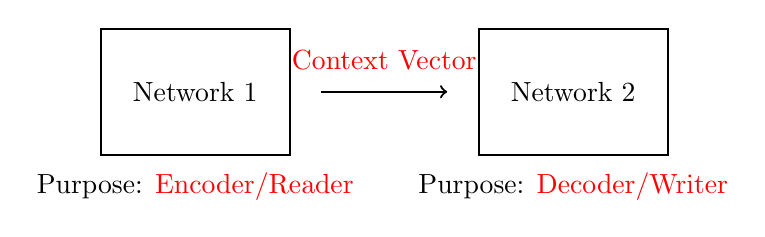
\begin{tikzpicture}[scale=0.8]
    % First network
    \draw[thick] (0,0) rectangle (3,2);
    \node at (1.5,1) {Network 1};
    \node at (1.5,-0.5) {Purpose: \textcolor{red}{Encoder/Reader}};
    
    % Arrow
    \draw[->, thick] (3.5,1) -- (5.5,1);
    \node at (4.5,1.5) {\textcolor{red}{Context Vector}};
    
    % Second network  
    \draw[thick] (6,0) rectangle (9,2);
    \node at (7.5,1) {Network 2};
    \node at (7.5,-0.5) {Purpose: \textcolor{red}{Decoder/Writer}};
\end{tikzpicture}
\end{center}

Network 1 (Encoder): Reads and understands the input sequence\\
Network 2 (Decoder): Generates the output sequence\\
Connection: Fixed-size context vector containing the ``meaning''
}

\question{What should pass between the two networks (what goes in the ??? box)?}

\solution{
The context vector should contain:
\begin{itemize}
    \item Semantic meaning of the input
    \item Abstract representation (not word-specific)
    \item Fixed size (e.g., 256 or 512 dimensions)
    \item Think of it as the ``understanding'' or ``gist''
\end{itemize}
}

\discovery{
Congratulations! Students just invented the encoder-decoder architecture! 
Network 1 = Encoder (compresses input to understanding)
Network 2 = Decoder (generates output from understanding)
}

\section{Part 3: The Bottleneck Discovery (10 minutes)}

\subsection{Long Sentence Challenge}

\exercise{Try to translate this paragraph using your two-network system:}

\begin{tcolorbox}[colback=blue!5!white]
``The International Conference on Machine Learning, which is one of the premier venues for presenting research in machine learning and attracts submissions from researchers around the world working on various aspects of learning algorithms, accepted our paper about using neural networks for natural language understanding, specifically focusing on how attention mechanisms can improve translation quality.''
\end{tcolorbox}

\question{If you compress this entire paragraph into a fixed-size vector (say, 256 numbers), what information might you lose?}

\solution{
Information loss by position:
\begin{itemize}
    \item Beginning: Conference name, ``premier venue'' detail
    \item Middle: ``researchers around the world'', ``various aspects''
    \item End: ``attention mechanisms'', ``translation quality'' specifics
    \item Overall: Lose sequential structure, specific relationships between clauses
\end{itemize}

This demonstrates that a fixed-size bottleneck loses information proportional to input length!
}

\think{This is like trying to remember an entire book by storing it as a single ``feeling'' - you'll forget the details!}

\subsection{Information Theory}

\question{Calculate the information loss:}

\solution{
\begin{itemize}
    \item Short sentence (5 words) compressed to 256 numbers: \underline{Minimal} loss
        \begin{itemize}
            \item Ratio: 256/5 = 51.2 numbers per word (plenty!)
        \end{itemize}
    \item Long document (500 words) compressed to 256 numbers: \underline{Massive} loss
        \begin{itemize}
            \item Ratio: 256/500 = 0.512 numbers per word (not enough!)
        \end{itemize}
\end{itemize}
}

\question{What's the fundamental problem here?}

\solution{
The fundamental problem is the \textbf{information bottleneck}:
\begin{itemize}
    \item Fixed-size representation regardless of input length
    \item Information capacity doesn't scale with input size
    \item Longer sequences = more compression = more loss
    \item This is why early seq2seq models failed on long sentences!
\end{itemize}
}

\discovery{
Students have identified the information bottleneck! Fixed-size representations can't capture all the information from arbitrarily long sequences.
}

\section{Part 4: Inventing Attention (15 minutes)}

\subsection{Human Translation Process}

\exercise{Translate this sentence step by step, marking which English words you look at for each French word:}

English: ``The black cat sat on the mat''

\solution{
\begin{center}
\begin{tabular}{|l|l|}
\hline
\textbf{Generating French word} & \textbf{Looking at English words} \\
\hline
``Le'' & \textcolor{red}{The} \\
``chat'' & \textcolor{red}{cat} \\
``noir'' & \textcolor{red}{black} \\
``s'est assis'' & \textcolor{red}{sat} \\
``sur'' & \textcolor{red}{on} \\
``le'' & \textcolor{red}{the} (second one) \\
``tapis'' & \textcolor{red}{mat} \\
\hline
\end{tabular}
\end{center}

Key insight: We don't look at all words equally - we focus on relevant parts for each output word!
}

\think{Notice how you don't look at ALL words equally - you focus on relevant parts!}

\subsection{Designing the Looking-Back Mechanism}

\question{Instead of compressing everything into one vector, what if the decoder could ``look back'' at all encoder states? Design a mechanism:}

\solution{
\begin{enumerate}
    \item How would you decide which encoder states are relevant?
        \begin{itemize}
            \item \textcolor{red}{Compare current decoder state with each encoder state}
            \item \textcolor{red}{Use similarity (dot product or learned function)}
            \item \textcolor{red}{Higher similarity = more relevant}
        \end{itemize}
    
    \item How would you combine multiple relevant states?
        \begin{itemize}
            \item \textcolor{red}{Weighted average based on relevance scores}
            \item \textcolor{red}{More relevant states get higher weights}
        \end{itemize}
    
    \item How would you turn this into weights that sum to 1?
        \begin{itemize}
            \item \textcolor{red}{Apply softmax to similarity scores}
            \item \textcolor{red}{This gives probability distribution over encoder states}
        \end{itemize}
\end{enumerate}

Congratulations! Students just invented the attention mechanism!
}

\subsection{Computing Attention Scores}

\exercise{For the word ``chat'' (cat), assign relevance scores (0-1) to each English word:}

\solution{
\begin{center}
\begin{tabular}{|l|c|}
\hline
\textbf{English word} & \textbf{Relevance to ``chat''} \\
\hline
The & \textcolor{red}{0.05} \\
black & \textcolor{red}{0.10} \\
cat & \textcolor{red}{0.70} \\
sat & \textcolor{red}{0.05} \\
on & \textcolor{red}{0.03} \\
the & \textcolor{red}{0.02} \\
mat & \textcolor{red}{0.05} \\
\hline
\textbf{Total} & \textcolor{red}{1.00} \\
\hline
\end{tabular}
\end{center}

Teaching points:
\begin{itemize}
    \item ``cat'' gets highest weight (0.70) - direct translation
    \item ``black'' gets some weight (0.10) - modifier that might influence
    \item Other words get minimal weight - not directly relevant
    \item Weights sum to 1.0 (probability distribution)
\end{itemize}
}

\discovery{
Students just invented attention! The relevance scores are attention weights, and looking back at all encoder states based on relevance is exactly how attention works!
}

\section{Part 5: Putting It All Together (10 minutes)}

\subsection{Complete Architecture}

Draw the complete sequence-to-sequence model with attention:

\solution{
Key components students should include:
\begin{enumerate}
    \item \textbf{Encoder:}
        \begin{itemize}
            \item Processes input words sequentially
            \item Produces hidden state for each word
            \item Keeps ALL hidden states (not just final)
        \end{itemize}
    
    \item \textbf{Attention Mechanism:}
        \begin{itemize}
            \item Compares decoder state to all encoder states
            \item Computes attention weights (softmax of similarities)
            \item Creates context vector (weighted sum)
        \end{itemize}
    
    \item \textbf{Decoder:}
        \begin{itemize}
            \item Generates output words one at a time
            \item Uses both its own state AND attention context
            \item Can ``look back'' at relevant input parts
        \end{itemize}
\end{enumerate}
}

\subsection{Key Components Checklist}

Check off each component you included:
\solution{
All boxes should be checked:
\begin{itemize}
    \item[\checkmark] Encoder network (processes input)
    \item[\checkmark] Multiple encoder hidden states (not just final)
    \item[\checkmark] Decoder network (generates output)
    \item[\checkmark] Attention mechanism (looks back at encoder states)
    \item[\checkmark] Attention weights (relevance scores)
    \item[\checkmark] Context vector (weighted sum)
\end{itemize}
}

\subsection{Reflection Questions}

\question{Why is attention better than a fixed-size bottleneck?}

\solution{
Attention solves the bottleneck problem by:
\begin{itemize}
    \item No information compression - keeps all encoder states
    \item Dynamic information access - decoder chooses what's relevant
    \item Scales with input length - longer inputs have more states to attend to
    \item Preserves fine details - can look back at specific words
    \item Handles long-range dependencies - can attend to distant words
\end{itemize}
}

\question{What tasks besides translation could benefit from this architecture?}

\solution{
Students might suggest:
\begin{itemize}
    \item Text summarization (attend to important parts)
    \item Question answering (attend to relevant context)
    \item Image captioning (attend to image regions)
    \item Speech recognition (attend to audio segments)
    \item Code generation (attend to specifications)
    \item Any task mapping sequences to sequences!
\end{itemize}
}

\question{What limitations might this approach still have?}

\solution{
Limitations to discuss:
\begin{itemize}
    \item Still sequential processing (slow)
    \item Attention computation scales O(n²) with sequence length
    \item RNN-based encoders still have gradient problems
    \item Fixed attention mechanism (not learnable enough)
    \item These limitations lead to Transformers (Week 5)!
\end{itemize}
}

\section{Bonus Challenge: Beam Search}

\think{When generating translations, should we always pick the most likely next word?}

\exercise{Consider translating ``bank'' - it could mean financial institution or river bank. Design a strategy to explore multiple translation paths:}

\solution{
Beam Search strategy:
\begin{itemize}
    \item Keep top-k translation hypotheses at each step (e.g., k=3)
    \item For ``bank'':
        \begin{itemize}
            \item Path 1: ``banque'' (financial) with probability 0.6
            \item Path 2: ``rive'' (river bank) with probability 0.3
            \item Path 3: ``bord'' (edge) with probability 0.1
        \end{itemize}
    \item Expand each path, keep top-k overall
    \item Final: Choose highest probability complete sentence
    \item This avoids getting stuck with early bad choices!
\end{itemize}
}

\hrule
\vspace{1em}

\section*{Teaching Notes}

\subsection{Timing Guidelines}
\begin{itemize}
    \item Part 1: 10 minutes - Focus on length mismatch problem
    \item Part 2: 15 minutes - Let students struggle with compression
    \item Part 3: 10 minutes - Make bottleneck problem visceral
    \item Part 4: 15 minutes - Guide toward attention naturally
    \item Part 5: 10 minutes - Consolidate understanding
\end{itemize}

\subsection{Common Student Misconceptions}
\begin{enumerate}
    \item \textbf{``Just use a bigger vector''} - Explain that any fixed size eventually fails
    \item \textbf{``Store all words separately''} - Good intuition! This leads toward attention
    \item \textbf{``Use multiple networks''} - Interesting, but coordination becomes complex
    \item \textbf{``Attention looks at future words''} - Clarify it only looks at input (encoder) states
\end{enumerate}

\subsection{Key Pedagogical Moments}
\begin{itemize}
    \item When students realize word-by-word fails - validate this discovery
    \item During compression exercise - let them experience information loss
    \item When inventing attention - connect to how humans translate
    \item Final assembly - celebrate that they invented a real system!
\end{itemize}

\section*{Summary}

Today students discovered:
\begin{enumerate}
    \item The variable-length challenge in translation
    \item The encoder-decoder architecture
    \item The information bottleneck problem
    \item The attention mechanism
\end{enumerate}

These concepts they ``invented'' are the foundation of modern machine translation systems like Google Translate!

\vspace{2em}
\noindent\textbf{Next Week:} We'll see how taking attention to the extreme (attention is ALL you need) leads to Transformers!

\end{document}